{
\titlegraphic{
  
\includegraphics[
    width=\paperwidth]{placeholder_yellow}
}
\title{\LaTeX{} Beamer Theme ``Juelich''}
\subtitle{Tutorial for the JSC Guest Student Programme}
\author{The GSP Organizers}
\institute[JSC]{Jülich Supercomputing Centre}
\date{\today}
\maketitle

\begin{frame}
        \frametitle{How to use the Jülich Theme}
        \framesubtitle{Parts of this Mini-Tutorial}
        \begin{itemize}
          \item \hyperlink{examples}{Part 1: Examples}
          \item \hyperlink{colors}{Part 2: Jülich Colors}
          \item \hyperlink{localization}{Part 3: Localization}
          \item \hyperlink{tweaks}{Part 4: Tweaks}
          \item \hyperlink{handouts}{Part 5: Handouts}
    \end{itemize}
\end{frame}

\part{Examples}
\makepart
\section{Features}
\selectlanguage{english}
\begin{frame}
        \frametitle{\LaTeX{}-Beamer Features}
        The following slides show how {\tt Latex-Beamer} constructs work within the
        template.
        \begin{itemize}
      %\item Framebreaks
      \item Lists, numbered lists
      \item Plain slides, background images
      \item Theorems, proofs
      \item Definitions, examples
      \item Blocks, alert blocks
      \item Highlight options
      \item Formulae
      \item Verbatim environments
    \end{itemize}
\end{frame}

\section{Lists}
\begin{frame}
        \frametitle{Lots of lists}
        \framesubtitle{Another Subtitle}
        \begin{itemize}
          \item using the \texttt{pause} command:
          \begin{itemize}
            \item First item.
            \pause
            \item Second item.
          \end{itemize}
          \item using overlay specifications:
          \begin{enumerate}
            \item<3-> First numbered item.
            \item<4-> Second numbered item.
            \begin{itemize}
              \item 3rd level item!
            \end{itemize}
          \end{enumerate}
          \item using the general \texttt{uncover} command:
          \begin{itemize}
            \uncover<5->{\item First item.}
            \uncover<6->{\item Second item.}
          \end{itemize}
        \end{itemize}
\end{frame}

\begin{frame}[fragile]
        \frametitle{Plain Frames}
        \begin{itemize}
      \item The next slide shows a plain frame.
      \item To use plain frames add the \verb![plain]! parameter to your \verb!\begin{frame}! statement.
    \end{itemize}
        \begin{block}{How to use plain frames}
    \scriptsize
    \verbatiminput{frame_plain}
        \end{block}
\end{frame}

%\begin{frame}[plain]
    \frametitle{Plain Frame}
    \begin{center}
        Here is my tiny text on a plain frame.
    \end{center}
\end{frame}


\begin{frame}[c,plain]
        \frametitle{Plain Frame}
        \begin{center}
                {\tiny Enough} {\scriptsize space} for {\Large your} {\huge big} {\Huge ideas.} {\TINY (or holiday pictures)}
        \end{center}
\end{frame}

\section{Backgrounds}
\begin{frame}[fragile]
    \frametitle{Background Images}
    \framesubtitle{On Standard Frames}
    \begin{itemize}
      \item The next slide shows an image, embedded into the background of the frame layout.
      \item The background image is automatically cropped to the frame dimensions.
    \end{itemize}
    \begin{block}{How to install a background image}
        \scriptsize
        \verbatiminput{frame_background}
    \end{block}
\end{frame}

\setbeamertemplate{background}{
\includegraphics[width=\paperwidth]{placeholder}}
\begin{frame}
    \frametitle{An image in the background}
    \centering
    Some text in front of the background image.
\end{frame}
\setbeamertemplate{background}{}


\section{Beamer Block Constructs}
\subsection{Theorem, Proof}
\begin{frame}
        \frametitle{Block Constructs}
        \framesubtitle{{\tt theorem, proof}}
        \begin{theorem}
        There is no largest prime number.
        \end{theorem}

        \begin{proof}
                \begin{enumerate}
                        \item<1-| alert@1> Suppose $p$ were the largest prime number.
                        \item<2-> Let $q$ be the product of the first $p$ numbers.
                        \item<3-> Then $q+1$ is not divisible by any of them.
                        \item<1-> Thus $q+1$ is also prime and greater than $p$.\qedhere
                \end{enumerate}
        \end{proof}
\end{frame}

\subsection{Definition, Example}
\begin{frame}
        \frametitle{Block Constructs}
        \framesubtitle{{\tt definition, example}}
        \begin{definition}
                A \alert{prime number} is a number that has exactly two divisors.
        \end{definition}
        \begin{example}
                \begin{itemize}
                        \item 2 is prime (two divisors: 1 and 2).
                        \item 3 is prime (two divisors: 1 and 3).
                        \item 4 is not prime (\alert{three} divisors: 1, 2, and 4).
                \end{itemize}
        \end{example}
\end{frame}

\subsection{Block, Alert Block}
\begin{frame}
        \frametitle{Block Constructs}
        \framesubtitle{{\tt block, alertblock}}
        \begin{block}{Simple Block}
                Just some text.
        \end{block}
        \begin{alertblock}{Alert Block}
                This block seems to be pretty important.
        \end{alertblock}
\end{frame}

\section{Highlight important information}
\begin{frame}[fragile]
        \frametitle{Highlight important information}
        \framesubtitle{Use ``Jülich'' colors to attract attention}
        \begin{block}{Use {\tt \textbackslash{}emph\{\}}}
                \verb+This text is \emph{important}.+ \\
                This text is \emph{important}.
        \end{block}
        \begin{block}{Use {\tt \textbackslash{}alert\{\}}}
                \verb+This text is \alert{really} important!+ \\
                This text is \alert{really} important!
        \end{block}
\end{frame}

\section{Math Environment}
\begin{frame}
        \frametitle{Math Environment}
        \framesubtitle{Use your {\LaTeX} formulae inside your slides without hassle}
        \[
            \iiint\limits_V \operatorname{div} \vec{F} \, dV
            = \iint\limits_S \vec{F}\cdot d\vec{S}
        \]
        \[
         \prod_{k=1}^n k = n! \,,\quad \sum_{k=1}^n k=\frac{n(n+1)}{2}\,,
          \quad \int_0^{2\pi}\sin t\,dt=0
        \]
        \[
            p(x)=\sum_{i=0}^n f_{i}q_{i}(x) \quad\mbox{with}\quad
            q_{i}(x)=\prod_{\substack{k=0 \\ k\neq i}}^n
            \frac{x-x_{k}}{x_{i}-x_{k}}\,.
        \]
        \[
            \iint\limits_S (U \operatorname{grad} W)\cdot d\vec{S}
            =\iiint\limits_V (\operatorname{grad} U\cdot
             \operatorname{grad} W +U\Delta W)\,dV
        \]
\end{frame}

\section{Code Environment}
\begin{frame}[fragile]
        \frametitle{Verbatim Environment}
        \framesubtitle{Code Snippets}
        \begin{itemize}
      \item Slides containing \verb!\verb! statements must be defined \verb+fragile+
    \end{itemize}
    \scriptsize
    \verbatiminput{frame_verbatim}
\end{frame}

\begin{frame}[fragile]
    \frametitle{Hello World in Intercal}
    \begin{verbatim}
        DO ,1 <- #13
        PLEASE DO ,1 SUB #1 <- #234
        DO ,1 SUB #2 <- #112
        DO ,1 SUB #3 <- #112
        DO ,1 SUB #4 <- #0
        DO ,1 SUB #5 <- #64
        DO ,1 SUB #6 <- #194
        DO ,1 SUB #7 <- #48
        PLEASE DO ,1 SUB #8 <- #22
        DO ,1 SUB #9 <- #248
        DO ,1 SUB #10 <- #168
        DO ,1 SUB #11 <- #24
        DO ,1 SUB #12 <- #16
        DO ,1 SUB #13 <- #214
        PLEASE READ OUT ,1
        PLEASE GIVE UP
    \end{verbatim}
\end{frame}


\newenvironment{fragileframe}%
  {\begin{frame}[fragile,environment=fragileframe]}%
  {\end{frame}}

\section{Backgrounds}
\begin{fragileframe}
        \frametitle{Background Images}
        \framesubtitle{On Standard Frames}
        \begin{itemize}
      \item The next slide shows an image, embedded into the background of the frame layout.
      \item The background image is automatically cropped to the frame dimensions.
    \end{itemize}
        \begin{block}{How to install a background image}
        \tiny
        \begin{verbatim}
                \setbeamertemplate{background}{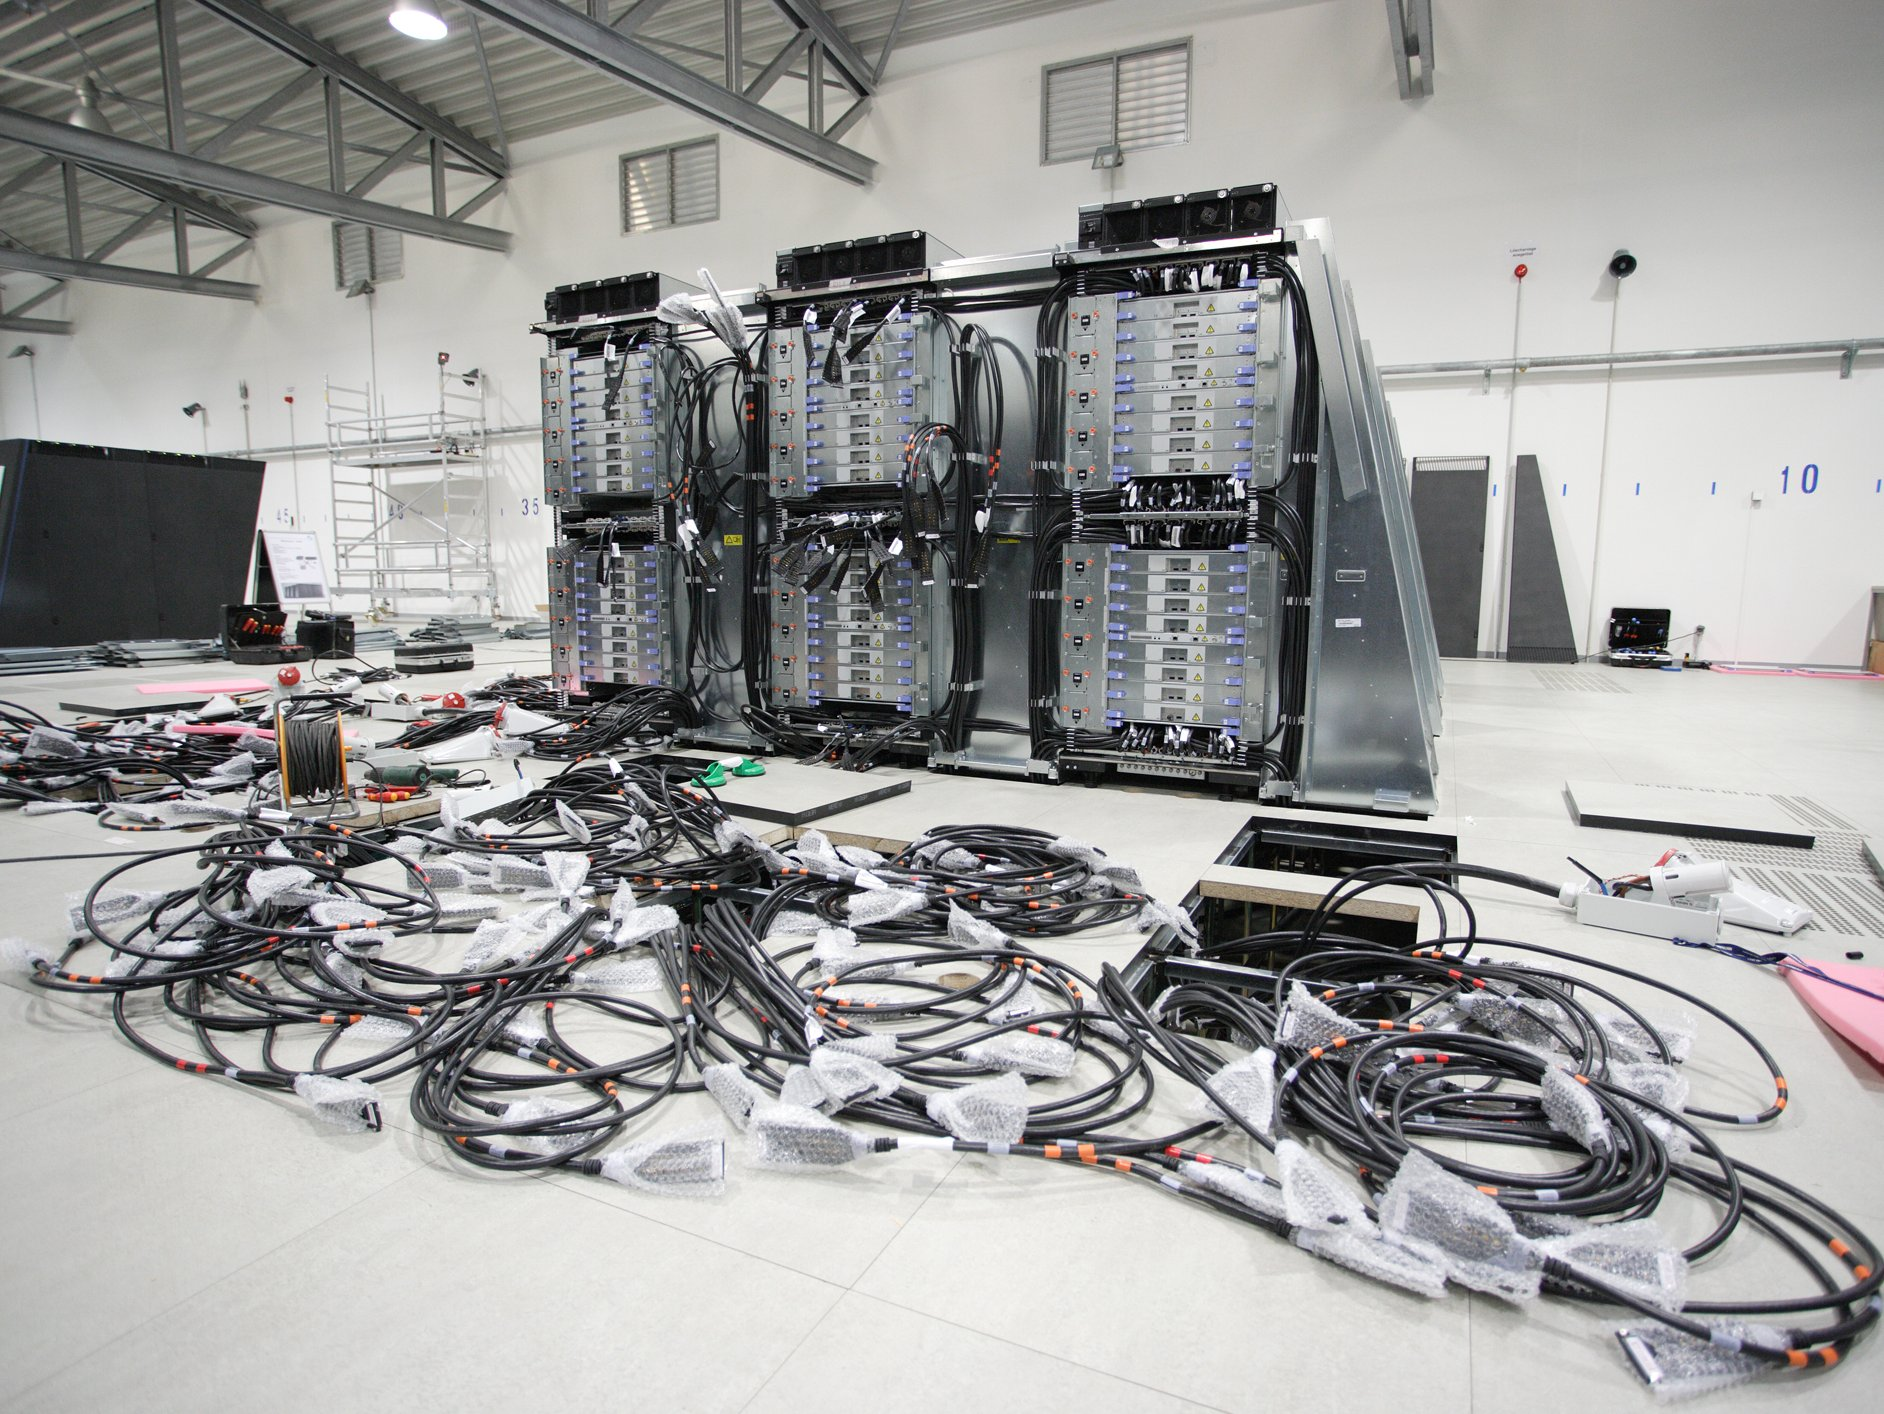
\includegraphics[width=\paperwidth]{background}}
                \begin{frame}
          Some text in front of the background image.
                \end{frame}
                \setbeamertemplate{background}{}
        \end{verbatim}
        \end{block}
\end{fragileframe}

\setbeamertemplate{background}{\includegraphics[width=\paperwidth]{lageplan}}
\begin{frame}
        \frametitle{Jülich Campus in the background}
        \vspace{5em}
        \centering
        \colorbox{fzjviolet}{\textcolor{fzjlightblue}{Some text in front of the background image.}}
\end{frame}
\setbeamertemplate{background}{}

\begin{fragileframe}
        \frametitle{Background Images}
        \framesubtitle{On Plain Frames}
        \begin{itemize}
          \item Use \verb!background canvas! instead of \verb!background! to flood fill a plain slide
          \item Again, the image is cropped to the frame boundaries
        \end{itemize}
        \begin{block}{How to install a background canvas image}
        \tiny
        \begin{verbatim}
                \setbeamertemplate{background canvas}{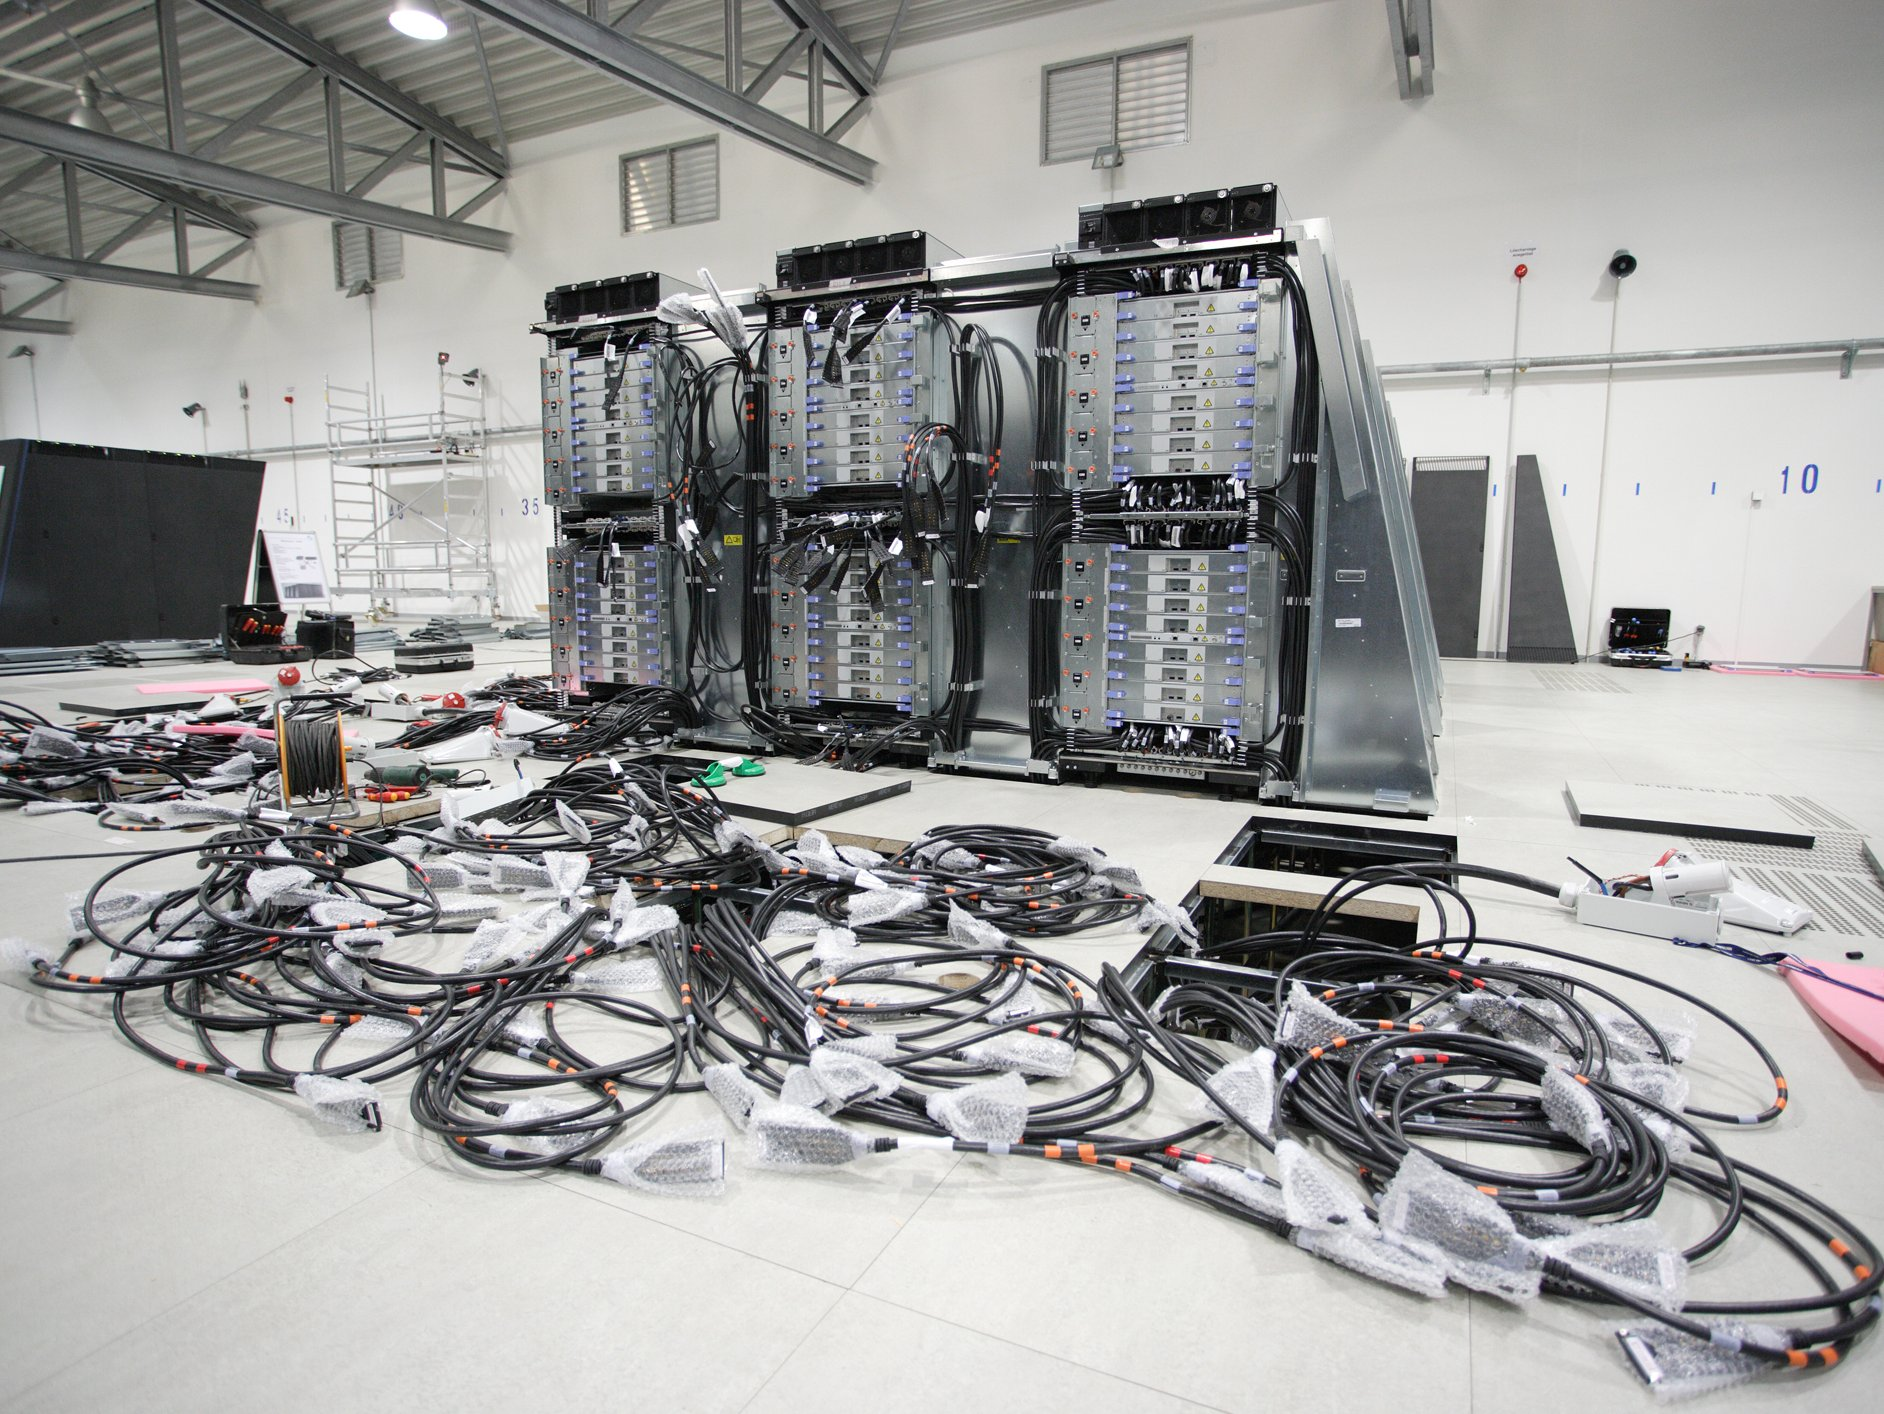
\includegraphics[width=\paperwidth]{background}}
                \begin{frame}[plain]
                \end{frame}
                \setbeamertemplate{background canvas}{}
        \end{verbatim}
        \end{block}
\end{fragileframe}

\setbeamertemplate{background canvas}{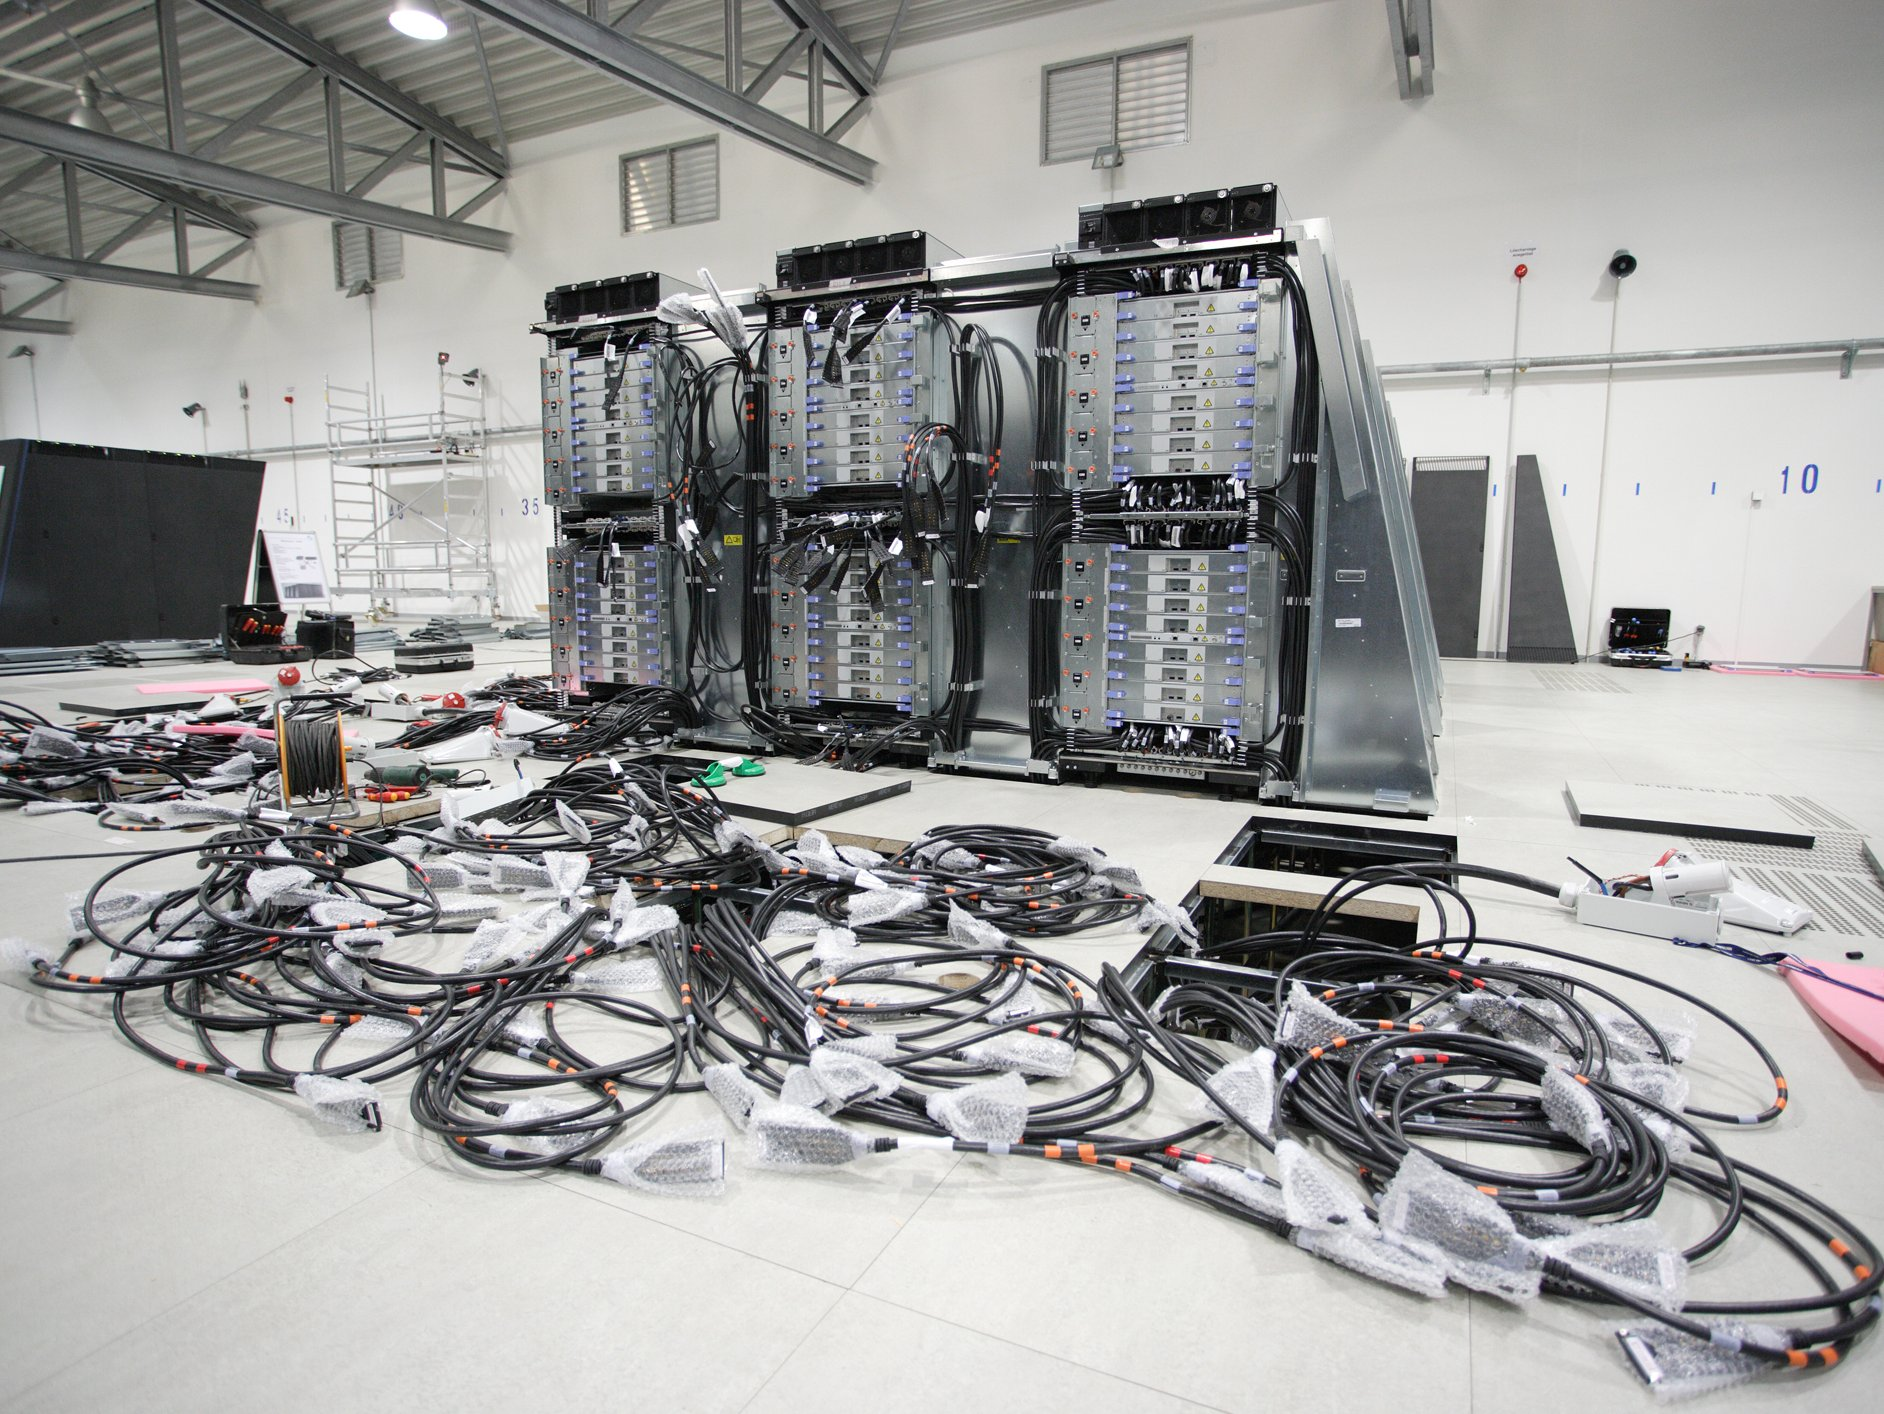
\includegraphics[width=\paperwidth]{background}}
\begin{frame}[plain]
\end{frame}
\setbeamertemplate{background canvas}{}

\begin{fragileframe}
        \begin{exampleblock}{Example Block}
                Just some text.
        \end{exampleblock}
        \begin{block}{Redefine commands with fancy colors}
                \verb+\renewcommand{\emph}[1]{\structure{#1}}+ \\
                Gives a nice blue text with every \verb+\emph{}+ command.
        \end{block}
\end{fragileframe}


\begin{comment}
\section{Split long text}
\begin{frame}[allowframebreaks,t]
        \frametitle{Automatically split long text}
        \framesubtitle{{\tt Beamer} can split text/lists to fit information on several
        slides}

        Lorem ipsum dolor sit amet, consetetur sadipscing elitr, sed diam nonumy eirmod
        tempor invidunt ut labore et dolore magna aliquyam erat, sed diam voluptua. At
        vero eos et accusam et justo duo dolores et ea rebum. Stet clita kasd gubergren,
        no sea takimata sanctus est Lorem ipsum dolor sit amet. Lorem ipsum dolor sit
        amet, consetetur sadipscing elitr, sed diam nonumy eirmod tempor invidunt ut
        labore et dolore magna aliquyam erat, sed diam voluptua. At vero eos et accusam
        et justo duo dolores et ea rebum. Stet clita kasd gubergren, no sea takimata
        sanctus est Lorem ipsum dolor sit amet. Lorem ipsum dolor sit amet, consetetur
        sadipscing elitr, sed diam nonumy eirmod tempor invidunt ut labore et dolore
        magna aliquyam erat, sed diam voluptua. At vero eos et accusam et justo duo
        dolores et ea rebum. Stet clita kasd gubergren, no sea takimata sanctus est Lorem
        ipsum dolor sit amet.

        Duis autem vel eum iriure dolor in hendrerit in vulputate velit esse molestie
        consequat, vel illum dolore eu feugiat nulla facilisis at vero eros et accumsan
        et iusto odio dignissim qui blandit praesent luptatum zzril delenit augue duis
        dolore te feugait nulla facilisi. Lorem ipsum dolor sit amet, consectetuer
        adipiscing elit, sed diam nonummy nibh euismod tincidunt ut laoreet dolore magna
        aliquam erat volutpat.

        Ut wisi enim ad minim veniam, quis nostrud exerci tation ullamcorper suscipit
        lobortis nisl ut aliquip ex ea commodo consequat. Duis autem vel eum iriure dolor
        in hendrerit in vulputate velit esse molestie consequat, vel illum dolore eu
        feugiat nulla facilisis at vero eros et accumsan et iusto odio dignissim qui
        blandit praesent luptatum zzril delenit augue duis dolore te feugait nulla
        facilisi.
\end{frame}
\end{comment}

\section{Columns}

\begin{comment}
\begin{frame}[fragile]
\frametitle{Columns}
\framesubtitle{To structure information use columns}
without columns
\rule{\textwidth}{2mm}
\begin{block}{}
\rule{\textwidth}{2mm}
\end{block}

2 columns, t, defaults, .5
\begin{columns}[t]
  \begin{column}{.5\textwidth}
\rule{\textwidth}{2mm}
  \end{column}
  \begin{column}{.5\textwidth}
\rule{\textwidth}{2mm}
  \end{column}
\end{columns}

2 columns, t, onlytextwidth, .5
\begin{columns}[t,totalwidth=\textwidth]
  \begin{column}{.5\textwidth}
\rule{\textwidth}{2mm}
  \end{column}
  \begin{column}{.5\textwidth}
\rule{\textwidth}{2mm}
  \end{column}
\end{columns}

2 columns, t, onlytextwidth, .485
\begin{columns}[t,onlytextwidth]
  \begin{column}{.485\textwidth}
\rule{\textwidth}{2mm}
  \end{column}
  \begin{column}{.485\textwidth}
\rule{\textwidth}{2mm}
  \end{column}
\end{columns}

\begin{columns}[t,onlytextwidth]
  \begin{column}{.485\textwidth}
\rule{\textwidth}{2mm}
    \begin{block}{I am a column}
\rule{\textwidth}{2mm}
    \end{block}
  \end{column}
  \begin{column}{.485\textwidth}
\rule{\textwidth}{2mm}
    \begin{block}{I am a column}
\rule{\textwidth}{2mm}
    \end{block}
  \end{column}
\end{columns}
\end{frame}
\end{comment}

\begin{frame}[fragile]
\frametitle{Columns}
\framesubtitle{To structure information use columns}
\begin{columns}[onlytextwidth]%[t] missing
  \begin{column}{.485\textwidth}
    \begin{block}{I am column one}
      \begin{itemize}
        \item items as usual
        \item another item
      \end{itemize}
    \end{block}
  \end{column}
  \begin{column}{.485\textwidth}
    \begin{block}{I am column two}
      \dots
    \end{block}
  \end{column}
\end{columns}
\vspace{1ex}

Use \verb!\begin{columns}[t]! to align at the top

\begin{columns}[t,onlytextwidth]
  \begin{column}{.485\textwidth}
    \begin{block}{I am column one}
      \begin{itemize}
        \item items as usual
        \item another item
      \end{itemize}
    \end{block}
  \end{column}
  \begin{column}{.485\textwidth}
    \begin{block}{I am column two}
      \dots
    \end{block}
  \end{column}
\end{columns}
\end{frame}

\begin{frame}
\frametitle{Columns}
\framesubtitle{You can also use uneven distributions}
\begin{columns}[t, onlytextwidth]
  \begin{column}{.285\textwidth}
    \begin{block}{I am column one}
      \begin{itemize}
        \item items as usual
      \end{itemize}
    \end{block}
  \end{column}
  \begin{column}{.685\textwidth}
    \begin{block}{I am column two}
      \dots
    \end{block}
  \end{column}
\end{columns}
\end{frame}

\begin{frame}
\frametitle{Columns}
\framesubtitle{Do not use more than 3 columns}
\begin{columns}[t, onlytextwidth]
  \begin{column}{.31\textwidth}
    \begin{block}{I am column one}
      \dots
    \end{block}
  \end{column}
  \begin{column}{.31\textwidth}
    \begin{block}{I am column two}
      \dots
    \end{block}
  \end{column}
  \begin{column}{.31\textwidth}
    \begin{block}{I am column three}
      \dots
    \end{block}
  \end{column}
\end{columns}
\end{frame}

\section{Plots}

\begin{frame}
\frametitle{Use Pgfplots for Plotting}
\framesubtitle{Large, simple plot}
\begin{tikzpicture}
\begin{axis}[width=\textwidth, height=\textheight,cycle list name=fzjblue,]
\addplot+[smooth]{(x)};
\addplot+[smooth]{(x-1)};
\addplot+[smooth]{(x-2)};
\addplot+[smooth]{(x-3)};
\addplot+[smooth]{(x-4)};
\addplot+[smooth]{(x-5)};
\addplot+[smooth]{(x-6)};
\addplot+[smooth]{(x-7)};
\addplot+[smooth]{(x-8)};
\end{axis}
\end{tikzpicture}
\end{frame}

\begin{frame}
\frametitle{Use Pgfplots for Plotting}
\framesubtitle{Different Cycle List}
\begin{tikzpicture}
\begin{axis}[width=\textwidth, height=\textheight,cycle list name=fzjdiagram,]
\addplot+[smooth]{(x)};
\addplot+[smooth]{(x-1)};
\addplot+[smooth]{(x-2)};
\addplot+[smooth]{(x-3)};
\addplot+[smooth]{(x-4)};
\addplot+[smooth]{(x-5)};
\addplot+[smooth]{(x-6)};
\addplot+[smooth]{(x-7)};
\end{axis}
\end{tikzpicture}
\end{frame}

\begin{frame}
\frametitle{Use Pgfplots for Plotting}
\framesubtitle{Highlighting a curve}
\begin{tikzpicture}
\begin{axis}[width=\textwidth, height=\textheight]
\addplot[color=fzjblue,smooth]{sin(100*x)};
\addlegendentry{data}
\addplot[color=fzjblue!50!white,smooth]{cos(100*x+10)+1};
\addlegendentry{more data}
\addplot[color=fzjgreen!80!white,smooth,onslide=<2>{color=fzjred,smooth}]{sin(80*x+420)+0.5};
\addlegendentry{yet more data}
\addplot[color=fzjviolet!80!white,smooth]{sin(120*x)+2};
\addlegendentry{even more data}
\end{axis}
\end{tikzpicture}
\end{frame}

\begin{frame}
\frametitle{More Plots}
\begin{block}{More Information}
Take a look at the
\href{http://pgfplots.sourceforge.net/gallery.html}{\globe pgfplots gallery}.
\end{block}
\end{frame}

\begin{frame}
\frametitle{Present Data In Tables}
\pgfplotstabletypeset[
every even row/.style={
before row={\rowcolor{fzjblue!05!white}}},
every head row/.style={
before row=\toprule,after row=\midrule},
every last row/.style={
after row=\bottomrule},
]
{Plots/pgfplotstable.example1.dat}

\end{frame}


\part{Jülich Colors}
\makepart

\begin{frame}[label=colors]
  \frametitle{Corporate Colors}
  \framesubtitle{You can use predefined colornames to spice up your slides}
  \centering
  \begin{tikzpicture}
    \foreach \color [count=\i] in {fzjorange, fzjviolet, fzjyellow, fzjgreen, fzjred, fzjlightblue, fzjblue} {
        \node[fill=\color,circle,minimum size=2.3cm] at (-\i*360/7+90: 2.3cm) {\color};
    }
  \end{tikzpicture}
\end{frame}

\begin{frame}[fragile]
    \frametitle{Using Corporate Colors}
    In text:
    \begin{itemize}
        \item \verb+\textcolor{colorname-text}{text}+\\
            There is a \textcolor{fzjgreen}{green} word in this sentence.
        \item \verb+\colorbox{colorname-background}{content}+\\
            \colorbox{fzjorange}{This text is on an \textcolor{fzjred}{orange} background.}
        \item \verb+\fcolorbox{colorname-frame}{colorname-background}{content}+\\
            \fcolorbox{fzjblue}{fzjlightblue}{\textcolor{fzjviolet}{This colored text is in a colorful framed box.}}
    \end{itemize}

    In TikZ, pgfplots: use the named colors in any color specification.
\end{frame}

\part{Localization}
\makepart
\section{Change Language}
\begin{frame}[fragile,label=localization]
        \frametitle{Localization}
        \framesubtitle{How to change the date display to another language}
        The date will be adjusted automatically. You just have to use the {\tt babel}
        package with the desired language.
        \begin{block}{Date style -- Mixed}
                load package with DE and EN (default): \hfill \verb+\usepackage[ngerman,english]{babel}+\\
                choose German: \hfill \verb+\selectlanguage{ngerman}+\\
                choose English: \hfill \verb+\selectlanguage{english}+
        \end{block}
        \begin{block}{Date style -- German}
                01. Januar 2018 \hfill
                \verb+\selectlanguage{ngerman}+
        \end{block}
        \begin{block}{Date style -- English}
                January 01, 2018 \hfill
                \verb+\selectlanguage{english}+
        \end{block}

\end{frame}

\selectlanguage{ngerman}
\begin{frame}[fragile,,label=translation]
        \frametitle{Localization/Language}
        \framesubtitle{Change Helmholtz Banner Text}
        Using the \texttt{babel} package with the language option automatically sets
        the correct labels for the slide counter and Helmholtz banner.

        \begin{block}{Helmholtz Banner and Date in German}
        \begin{itemize}
          \item Take a look at the date and Helmholtz banner in the lower left
          corner and the slide name and frame number in the middle
          \item This slide should show the german version
          \item Enable options via \verb+\documentclass[english,ngerman]{beamer}+
          \item Enabled locally via \verb+\selectlanguage{ngerman}+ before
          \verb+\begin{frame}+
        \end{itemize}
        \end{block}
\end{frame}

\selectlanguage{english}
\author{Your Name}

\part{Tweaks}
\makepart
\section{Slide Number Display}

\begin{frame}[fragile,label=tweaks]
        \frametitle{Slide Number Display}
        \framesubtitle{How to change the slide number style}
        \begin{block}{Full Display: Current Slide | Overall Number of Slides}
                \scriptsize\verb+\setbeamertemplate{frame number}[full]+ \hfill
                \scriptsize\usebeamercolor[fg]{frametitle} Slide 42 $|$ 524
        \end{block}
        \begin{block}{No Display: empty}
                \scriptsize\verb+\setbeamertemplate{frame number}[empty]+ \hfill
                \scriptsize\usebeamercolor[fg]{frametitle}
        \end{block}
        \begin{block}{Default Display: Current Slide}
                \scriptsize\verb+\setbeamertemplate{frame number}[default]+ \hfill
                \scriptsize\usebeamercolor[fg]{frametitle} Slide 42
        \end{block}
        \begin{block}{Translation}
        If you choose german as language the name \emph{Slide} will be translated
        to \emph{Folie} automatically (See \hyperlink{translation}{\alert{this}}
        slide)
        \end{block}
\end{frame}

\section{Partner Logos}

\setbeamertemplate{footer element1}[logo]{jara}%
\setbeamertemplate{footer element3}[logo]{uni_bonn}%
\setbeamertemplate{footer element2}[logo]{rwth}%

\begin{frame}[fragile]
        \frametitle{Project Partners}
        \framesubtitle{How to set up partner logos}
        \begin{itemize}
      \item Show up to 3 partner logos, on this slide Jara, RWTH, Bonn
      \item Design your logos with sufficiently large white borders
      \item {pdf\LaTeX} pictures file types: \verb+.pdf .png .jpg+
    \end{itemize}
        \begin{block}{Show logos}
        \verb+\setbeamertemplate{footer element1}[logo]{jara}+
                \verb+\setbeamertemplate{footer element2}[logo]{uni_bonn}+
        \verb+\setbeamertemplate{footer element3}[logo]{rwth}+
    \end{block}
        \begin{block}{Reset back to default settings}
        \verb+\setbeamertemplate{footer element1}[default]+
        \verb+\setbeamertemplate{footer element2}[default]+
        \verb+\setbeamertemplate{footer element3}[default]+
    \end{block}
\end{frame}
\setbeamertemplate{footer element1}[default]
\setbeamertemplate{footer element2}[default]
\setbeamertemplate{footer element3}[default]

\part{Handouts}
\makepart
\section{Handouts}
\begin{frame}[fragile,label=handouts,t]
        \frametitle{Create Handouts}
        \begin{block}{Switch and Setup Render Mode}
     \scriptsize
                \verb+\documentclass[handout]{beamer}+\\
                        \verb+\mode<handout>{+\\
                        \verb+\pgfpagesuselayout{4 on 1}[a4paper,landscape,border shrink=5mm]}+
    \end{block}
        \begin{block}{Define Number of Pages per Sheet}
        \scriptsize
        \verb+\pgfpagesuselayout{2 on 1}[a4paper,border shrink=5mm]+
        \verb+\pgfpagesuselayout{4 on 1}[a4paper,landscape,border shrink=5mm]+
        \verb+\pgfpagesuselayout{8 on 1}[a4paper,border shrink=5mm]+
        \verb+\pgfpagesuselayout{16 on 1}[a4paper,landscape,border shrink=5mm]+
    \end{block}
        \begin{block}{Further Reading -- See {\tt Latex-Beamer} manual for details}
        {\scriptsize
        \url{http://www.ctan.org/tex-archive/macros/latex/contrib/beamer/doc/beameruserguide.pdf}}
    \end{block}
\end{frame}

\part{How To Do Bibliographies}
\begin{frame}
    \frametitle{How to Do References}
    \begin{itemize}
      \item My talk is interesting \cite{ref1}.
      \item But this paper shows how it is really done \cite{ref2}.
      \item Wow, these guys did stupid things \cite{ref3}.
      \item Cite figures in the caption below, or in the text aside.
      \item Put your references in \texttt{references.bib}
    \end{itemize}
\end{frame}

\section{References}
\begin{frame}[allowframebreaks]
\frametitle{References}
    \tiny{\bibliographystyle{alpha}}
    %\tiny{\bibliographystyle{unsrt}}
    \bibliography{references}
\end{frame}


}
